\documentclass[tikz,border=8pt]{standalone}
\usepackage{amsmath}
\usetikzlibrary{arrows.meta,calc}
\definecolor{ink}{HTML}{21352F}
\definecolor{teal}{HTML}{087F7B}
\definecolor{blue}{HTML}{4B77A8}
\definecolor{gold}{HTML}{C58B2A}
\definecolor{rose}{HTML}{B65A62}
\begin{document}
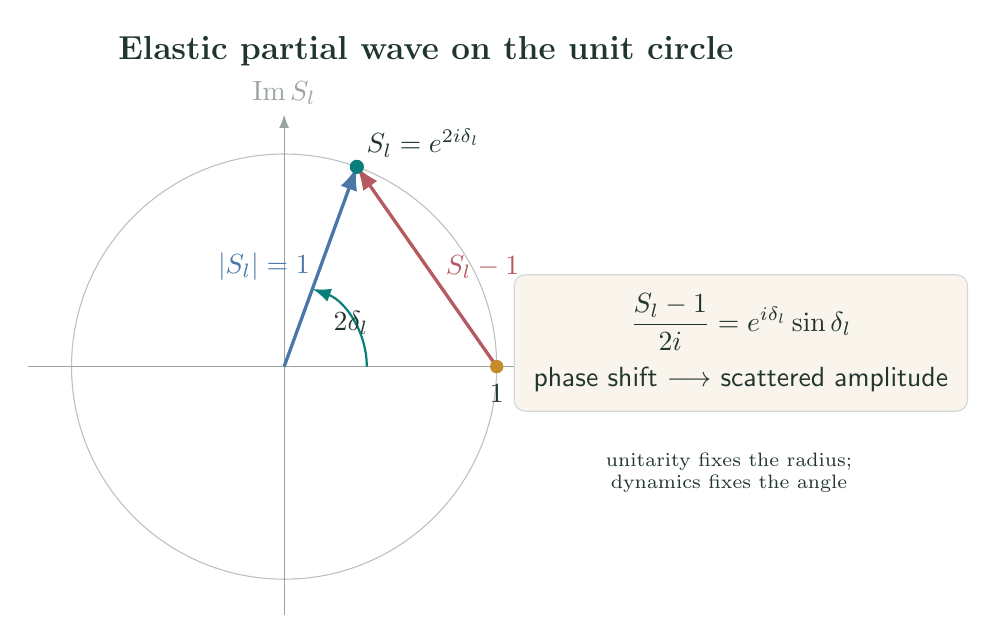
\begin{tikzpicture}[font=\sffamily,text=ink,>=Latex]
  \node[font=\bfseries\large] at (0,4.0)
    {Elastic partial wave on the unit circle};
  \coordinate (O) at (-1.8,0);
  \coordinate (I) at (.9,0);
  \coordinate (S) at ($(O)+(70:2.7)$);

  \draw[ink!30] (O) circle (2.7);
  \draw[->,ink!45] ($(O)+(-3.25,0)$)--($(O)+(3.45,0)$)
    node[right] {$\operatorname{Re}S_l$};
  \draw[->,ink!45] ($(O)+(0,-3.15)$)--($(O)+(0,3.2)$)
    node[above] {$\operatorname{Im}S_l$};
  \draw[blue,very thick,->] (O)--(S)
    node[midway,left] {$|S_l|=1$};
  \draw[rose,very thick,->] (I)--(S)
    node[midway,right=3pt] {$S_l-1$};
  \fill[gold] (I) circle (.085);
  \node[below=3pt] at (I) {$1$};
  \fill[teal] (S) circle (.09);
  \node[above right] at (S) {$S_l=e^{2i\delta_l}$};

  \draw[teal,thick,->] ($(O)+(1.05,0)$)
    arc[start angle=0,end angle=70,radius=1.05];
  \node at (-.95,.55) {$2\delta_l$};

  \node[draw=ink!20,fill=gold!9,rounded corners=4pt,
        inner sep=7pt,align=center] at (4.0,.3)
    {$\displaystyle
      \frac{S_l-1}{2i}
      =e^{i\delta_l}\sin\delta_l$\\[5pt]
     phase shift $\longrightarrow$ scattered amplitude};
  \node[font=\scriptsize,align=center] at (3.85,-1.35)
    {unitarity fixes the radius;\\
     dynamics fixes the angle};
\end{tikzpicture}
\end{document}
